\documentclass[conference]{IEEEtran}
\usepackage[utf8]{inputenc}
\usepackage[T1]{fontenc}
\usepackage{graphicx}
\usepackage{booktabs}
\usepackage{amsmath}
\usepackage{cite}
\usepackage{url}
\usepackage[hidelinks]{hyperref}

\graphicspath{{../figures/}}

\renewcommand{\figurename}{Gambar}
\renewcommand{\tablename}{Tabel}
\renewcommand{\abstractname}{Abstrak}
\renewcommand{\IEEEkeywordsname}{Kata kunci}
\renewcommand{\refname}{Referensi}

\newcommand{\dmean}{\ensuremath{\Delta}mean}
\newcommand{\dsd}{\ensuremath{\Delta}SD}
\newcommand{\dcount}{\ensuremath{\Delta}count}

\begin{document}

\title{Visualisasi dan Deteksi Anomali Jumlah Pemain Harian Game Steam Menggunakan Image Encoding dan Convolutional Neural Network}

\author{
\IEEEauthorblockN{Fahd Muhammad Zahid (13524078)}
\IEEEauthorblockA{Institut Teknologi Bandung\\Bandung, Indonesia}
\and
\IEEEauthorblockN{Ishaq Irfan Farizal (13524094)}
\IEEEauthorblockA{Institut Teknologi Bandung\\Bandung, Indonesia}
}

\maketitle

\begin{abstract}
Jumlah pemain harian sebuah game adalah data time series nyata yang naik turun karena tren jangka panjang, pola mingguan, dan lonjakan sesaat. Penelitian ini menerapkan metode Rahadian dkk. pada data jumlah pemain harian enam game Steam untuk mendeteksi anomali dengan mengubah segmen 20 hari menjadi gambar memakai 14 jenis image encoding (GADF, GASF, dan 12 varian MTF), lalu mengklasifikasikannya dengan convolutional neural network (CNN). Anomali dibuat dengan melipatgandakan atau membagi jumlah pemain pada 1 sampai 5 hari acak. Hasilnya, GADF dan GASF memberikan akurasi test tertinggi (97,8\% dan 97,3\%), sedangkan MTF Quantile paling rendah (56,5\% sampai 70,8\%). Visualisasi Grad-CAM menunjukkan bahwa pada segmen yang terdeteksi benar, CNN memperhatikan garis silang pada gambar GADF yang bersesuaian dengan hari anomali. Korelasi Pearson antara selisih simpangan baku matriks (\dsd) dan akurasi hanya 0,507, lebih lemah daripada 0,944 pada paper acuan, sehingga pada data ini pemilihan encoding cukup dari statistik matriks kurang dapat diandalkan. Data juga memperlihatkan pola mingguan yang konsisten: jumlah pemain pada Sabtu dan Minggu lebih tinggi daripada hari kerja di keenam game.
\end{abstract}

\begin{IEEEkeywords}
time series, deteksi anomali, Gramian Angular Field, Markov Transition Field, CNN, Grad-CAM
\end{IEEEkeywords}

\section{Pendahuluan}

Data time series muncul di banyak bidang, mulai dari sensor industri sampai aktivitas pengguna layanan digital. Salah satu contoh yang mudah diamati adalah jumlah pemain sebuah game pada platform Steam. Angka ini berubah setiap hari: naik saat game baru dirilis atau mendapat pembaruan besar, turun perlahan seiring waktu, dan berulang setiap pekan mengikuti kebiasaan pemain. Perubahan yang tidak biasa, misalnya lonjakan atau penurunan tajam dalam satu hari, dapat dianggap sebagai anomali yang menarik untuk dideteksi.

Rahadian dkk.~\cite{rahadian2023} menunjukkan bahwa anomali pada time series dapat dideteksi dengan mengubah potongan data menjadi gambar memakai Gramian Angular Field (GAF) dan Markov Transition Field (MTF), lalu mengklasifikasikan gambar tersebut dengan convolutional neural network (CNN). Paper tersebut juga menemukan bahwa selisih statistik matriks hasil encoding antara data normal dan anomali, terutama selisih simpangan baku (\dsd), berkorelasi sangat kuat dengan akurasi CNN, sehingga encoding yang baik dapat dipilih tanpa harus melatih CNN satu per satu.

Penelitian ini menerapkan metode yang sama pada data jumlah pemain harian enam game Steam. Tujuannya ada tiga. Pertama, memvisualisasikan data dan gambar hasil encoding untuk memperoleh insight tentang perilaku pemain. Kedua, membandingkan 14 jenis encoding dan melihat apakah temuan Rahadian dkk.\ juga berlaku pada data ini. Ketiga, memakai Grad-CAM~\cite{selvaraju2017} untuk melihat bagian gambar, dan karena itu hari, mana yang membuat CNN menganggap sebuah segmen anomali.
\section{Tinjauan Pustaka}

\subsection{Gramian Angular Field}
GAF mengubah time series $X=(x_1,\dots,x_n)$ menjadi matriks $n \times n$~\cite{wang2015}. Data terlebih dahulu diskalakan ke rentang $[-1,1]$, lalu tiap nilai diubah menjadi sudut $\phi_i=\arccos(\tilde{x}_i)$. Gramian Angular Summation Field (GASF) dan Gramian Angular Difference Field (GADF) didefinisikan sebagai
\begin{equation}
\mathrm{GASF}_{ij}=\cos(\phi_i+\phi_j), \qquad \mathrm{GADF}_{ij}=\sin(\phi_i-\phi_j).
\end{equation}
Setiap piksel $(i,j)$ menggambarkan hubungan antara titik waktu ke-$i$ dan ke-$j$, sehingga satu titik yang berubah akan mengubah satu baris dan satu kolom pada gambar.

\subsection{Markov Transition Field}
MTF membagi nilai time series ke dalam $Q$ kelompok (bin), menghitung peluang perpindahan dari satu bin ke bin lain pada titik waktu berurutan, lalu menyusun matriks $n\times n$ dengan $M_{ij}=w_{q(i)\,q(j)}$, yaitu peluang transisi antara bin titik ke-$i$ dan bin titik ke-$j$~\cite{wang2015}. Pustaka pyts~\cite{faouzi2020} menyediakan tiga cara pembagian bin: \textit{uniform} (lebar bin sama), \textit{quantile} (jumlah titik per bin sama), dan \textit{normal} (batas bin mengikuti kuantil distribusi normal baku).

\subsection{CNN dan Grad-CAM}
CNN mengenali pola pada gambar melalui lapisan konvolusi, pooling, dan lapisan terhubung penuh. Grad-CAM~\cite{selvaraju2017} menjelaskan keputusan CNN dengan menghitung bobot tiap peta fitur pada lapisan konvolusi terakhir dari rata-rata gradien keluaran terhadap peta fitur tersebut, lalu menjumlahkan peta fitur dengan bobot itu dan membuang nilai negatif. Hasilnya adalah peta panas yang menunjukkan area gambar yang paling mendorong keputusan.

\subsection{Statistik Matriks dan Korelasi Pearson}
Rahadian dkk.~\cite{rahadian2023} menghitung rata-rata (mean), simpangan baku (SD), dan jumlah nilai unik (count) dari setiap matriks hasil encoding. Nilai-nilai ini dirata-ratakan untuk seluruh data normal dan seluruh data anomali, lalu selisih absolutnya disebut \dmean, \dsd, dan \dcount. Kekuatan hubungan antara tiap selisih dan akurasi CNN diukur dengan koefisien korelasi Pearson $r$, yang bernilai antara $-1$ dan $1$.

\section{Metodologi}

\subsection{Data dan Pembersihan}
Data yang dipakai adalah jumlah pemain bersamaan (concurrent players) harian dari enam game Steam, yaitu Dark Souls 3, Euro Truck Simulator 2 (ETS2), Garry's Mod, Rainbow Six Siege, Stardew Valley, dan Terraria. Data diambil dari repositori Steam-Game-Analytics~\cite{steamrepo} yang bersumber dari SteamDB~\cite{steamdb}. Sebagian besar data tersedia per hari, kecuali sekitar satu bulan terakhir yang tersedia dalam interval 1 jam dan 10 menit. Bagian tersebut diseragamkan menjadi data harian dengan mengambil nilai maksimum setiap hari.

Beberapa langkah pembersihan dilakukan. Hari terakhir dibuang karena datanya belum lengkap. Nilai 1 sampai 3 pemain sebelum game dirilis dibuang dengan memulai data dari hari pertama yang memiliki minimal 1.000 pemain, sedangkan Garry's Mod dimulai dari 1 Januari 2012 karena data sebelumnya banyak yang hilang. Tanggal kosong hanya diisi dengan interpolasi linear jika celahnya paling lama tiga hari. Setelah pembersihan diperoleh 24.875 hari data. Dari 187 hari yang kosong, 6 hari diisi interpolasi dan 181 hari dibiarkan kosong.

\subsection{Segmentasi dan Anomali Buatan}
Setiap game dipotong menjadi segmen 20 hari yang tidak saling tumpang tindih, mengikuti panjang segmen pada paper acuan~\cite{rahadian2023}. Segmen yang masih mengandung hari kosong dilewati. Hasilnya adalah 1.229 segmen normal, terdiri atas 167 (Dark Souls 3), 220 (ETS2), 244 (Garry's Mod), 174 (Rainbow Six Siege), 170 (Stardew Valley), dan 254 (Terraria).

Data asli tidak memiliki label anomali, sehingga anomali dibuat seperti pada paper acuan. Untuk setiap segmen normal dibuat satu salinan anomali dengan memilih 1 sampai 5 hari secara acak. Jumlah pemain pada hari terpilih dikalikan dengan faktor acak antara 2 dan 5 (lonjakan) atau dibagi dengan faktor yang sama (penurunan), dengan arah yang dipilih acak untuk setiap hari. Suntikan dilakukan pada jumlah pemain asli. Setelah itu seluruh data diubah ke skala $\log_{10}$ dan distandarisasi per game, karena skala tiap game sangat berbeda.

Data dibagi menjadi 70\% train, 15\% validasi, dan 15\% test dengan seed tetap. Pembagian dilakukan per pasangan, sehingga segmen normal dan salinan anomalinya selalu berada di bagian yang sama. Rata-rata dan simpangan baku untuk standarisasi hanya dihitung dari segmen normal pada data train. Hasilnya adalah 860 pasangan train, 184 pasangan validasi, dan 185 pasangan test, atau 1.720, 368, dan 370 gambar.

\subsection{Image Encoding}
Setiap segmen diubah menjadi matriks $20\times20$ dengan 14 encoding dari pustaka pyts~\cite{faouzi2020}, yaitu GADF, GASF, serta MTF dengan strategi uniform, quantile, dan normal, masing-masing dengan 2, 4, 5, dan 10 bin. Parameter lain dibiarkan pada nilai bawaan seperti pada paper acuan. Matriks diubah menjadi gambar berwarna dengan colormap \textit{rainbow}, rentang warna $[-1,1]$ untuk GAF dan $[0,1]$ untuk MTF, lalu diperbesar menjadi $150\times150$ piksel.

\subsection{CNN}
Arsitektur CNN mengikuti paper acuan~\cite{rahadian2023}: tiga blok konvolusi dengan 16, 32, dan 64 filter berukuran $3\times3$, aktivasi ReLU, dan max pooling, diikuti lapisan dense 512 unit dan satu unit keluaran sigmoid. Model dilatih dengan optimizer RMSprop (learning rate 0,001), loss binary cross-entropy, batch 20, dan 20 epoch. Satu model dilatih untuk setiap encoding dengan pengaturan dan seed yang sama, tanpa penyesuaian khusus per encoding. Implementasi memakai PyTorch, dan model setelah epoch ke-20 yang dievaluasi pada data test.

\subsection{Analisis}
Nilai \dmean, \dsd, dan \dcount{} dihitung dari seluruh 1.229 pasangan segmen, lalu dikorelasikan dengan akurasi test CNN memakai korelasi Pearson pada 14 titik (satu per encoding). Grad-CAM diterapkan pada model dengan akurasi test tertinggi untuk beberapa segmen anomali pada data test. Peta panas dikembalikan ke ukuran matriks $20\times20$, lalu skor tiap hari dihitung sebagai jumlah nilai pada baris dan kolom hari tersebut.

\section{Hasil dan Pembahasan}

\subsection{Gambaran Data}

\begin{figure*}[t]
\centering
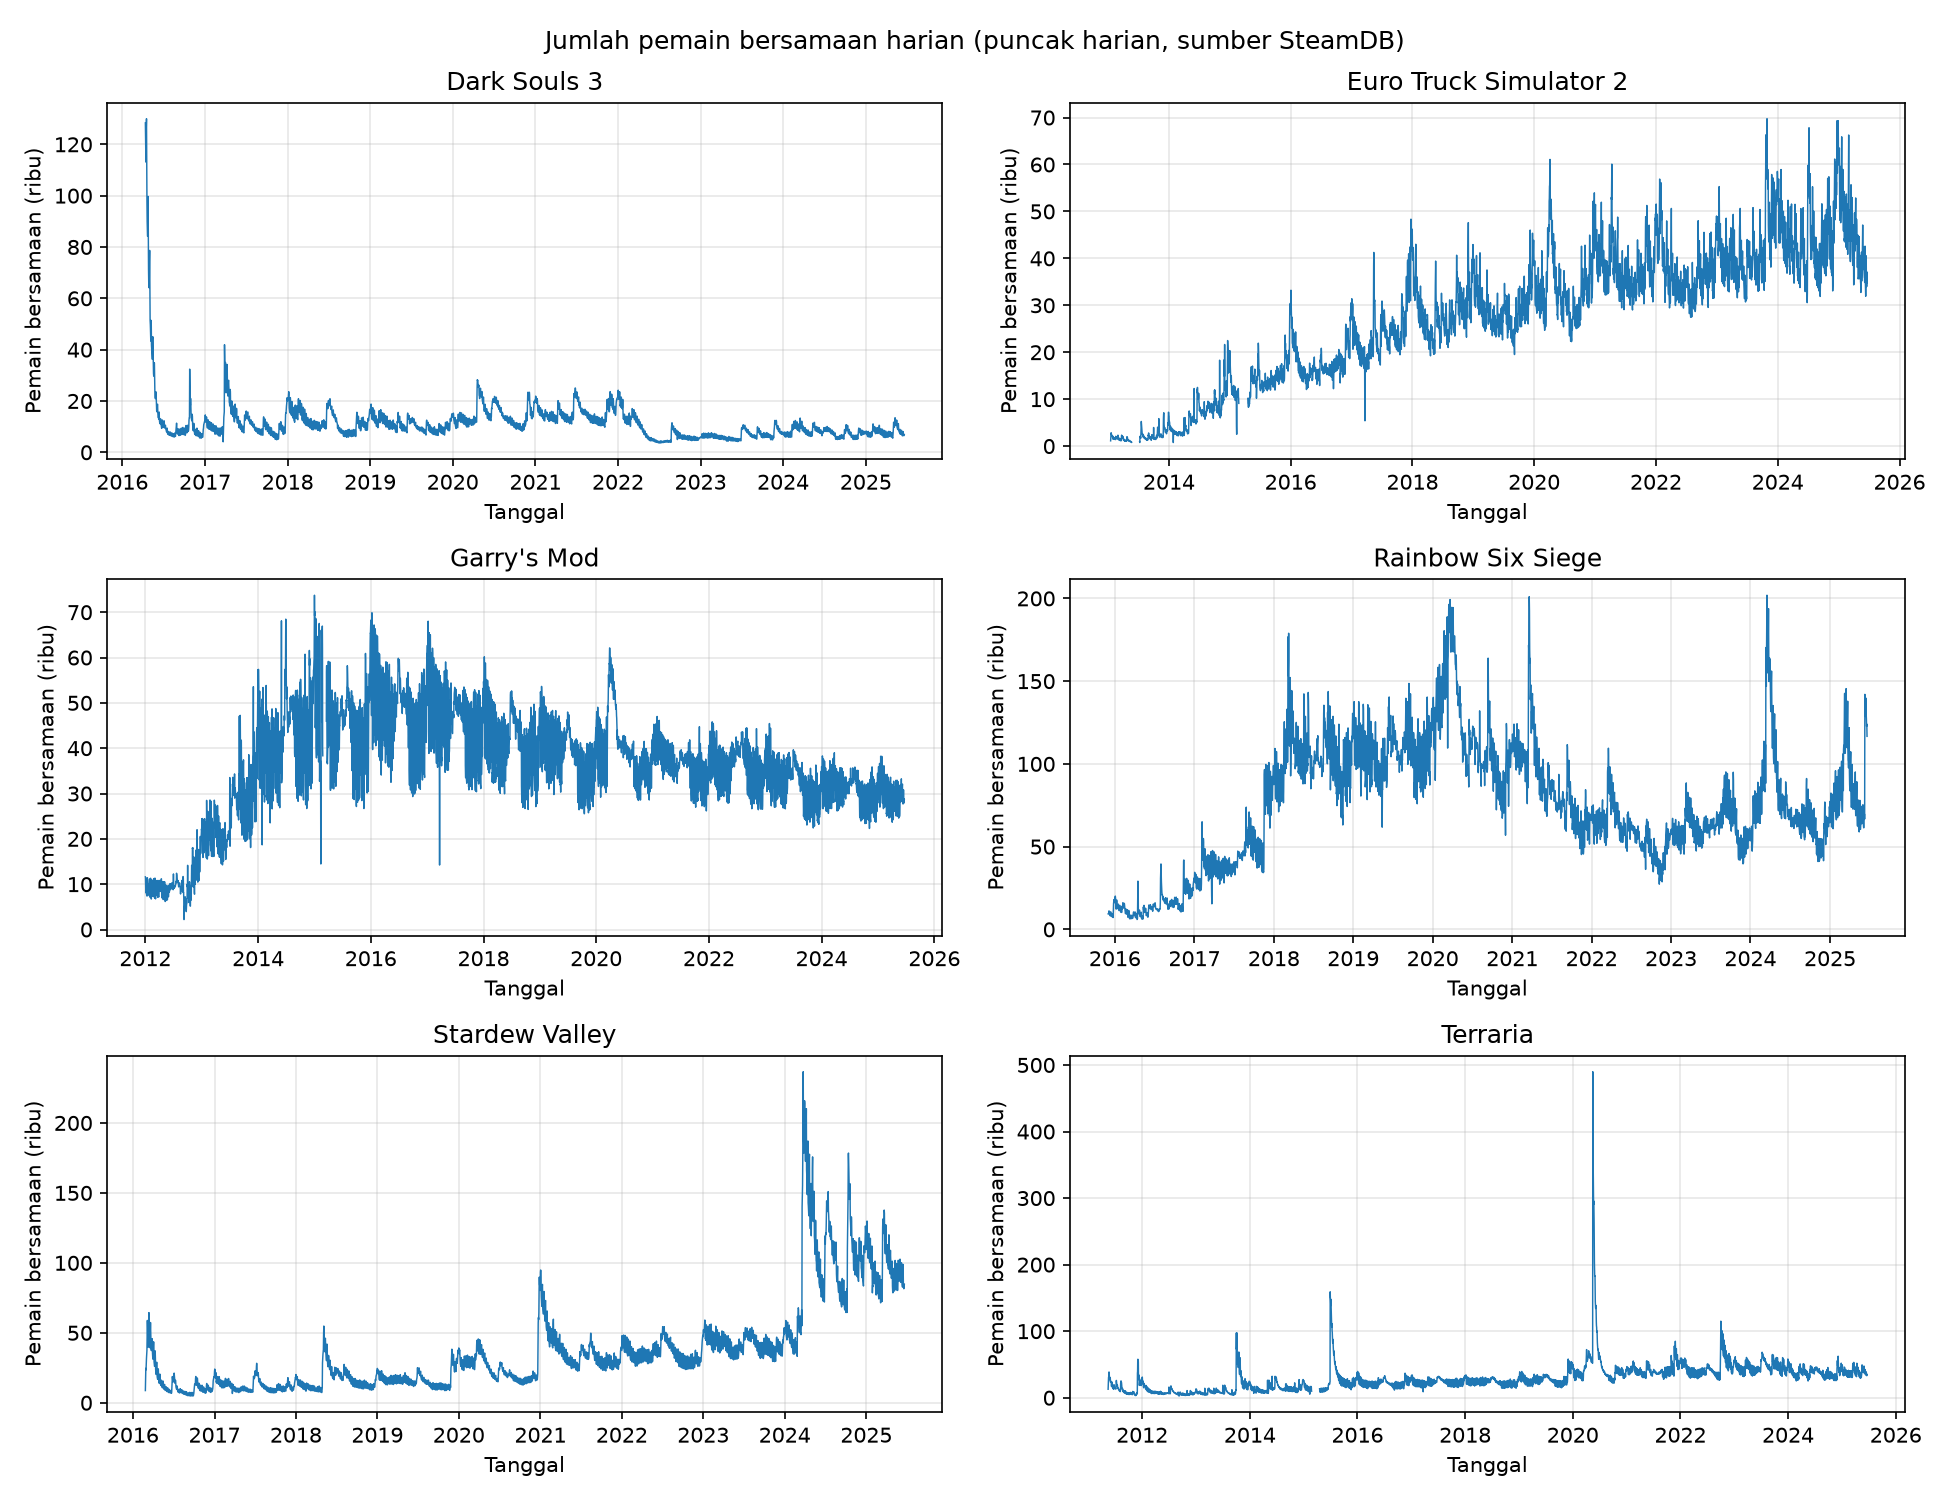
\includegraphics[width=0.58\textwidth]{01_pemain_harian.png}
\caption{Jumlah pemain bersamaan harian keenam game setelah pembersihan (sumber data: SteamDB~\cite{steamdb}).}
\label{fig:harian}
\end{figure*}

Gambar~\ref{fig:harian} memperlihatkan bahwa setiap game memiliki pola jangka panjang yang berbeda. Dark Souls 3 mencapai puncak pada awal rilis lalu turun dan stabil, ETS2 tumbuh hampir terus-menerus, sedangkan Rainbow Six Siege dan Stardew Valley naik turun dengan beberapa lonjakan besar. Terraria memiliki beberapa lonjakan yang sangat tinggi dibanding tingkat normalnya. Lonjakan seperti ini kemungkinan berkaitan dengan pembaruan besar atau event tertentu, namun penyebabnya tidak diverifikasi dalam penelitian ini.

Lonjakan alami juga terlihat pada tingkat segmen. Sebanyak 125 dari 1.229 segmen normal (10,2\%) sudah memuat satu hari dengan jumlah pemain lebih dari 1,5 kali median segmennya. Persentase tertinggi ada pada Terraria (20,1\%) dan terendah pada Rainbow Six Siege (5,2\%). Segmen-segmen ini tetap diperlakukan sebagai segmen normal.

\begin{figure}[t]
\centering
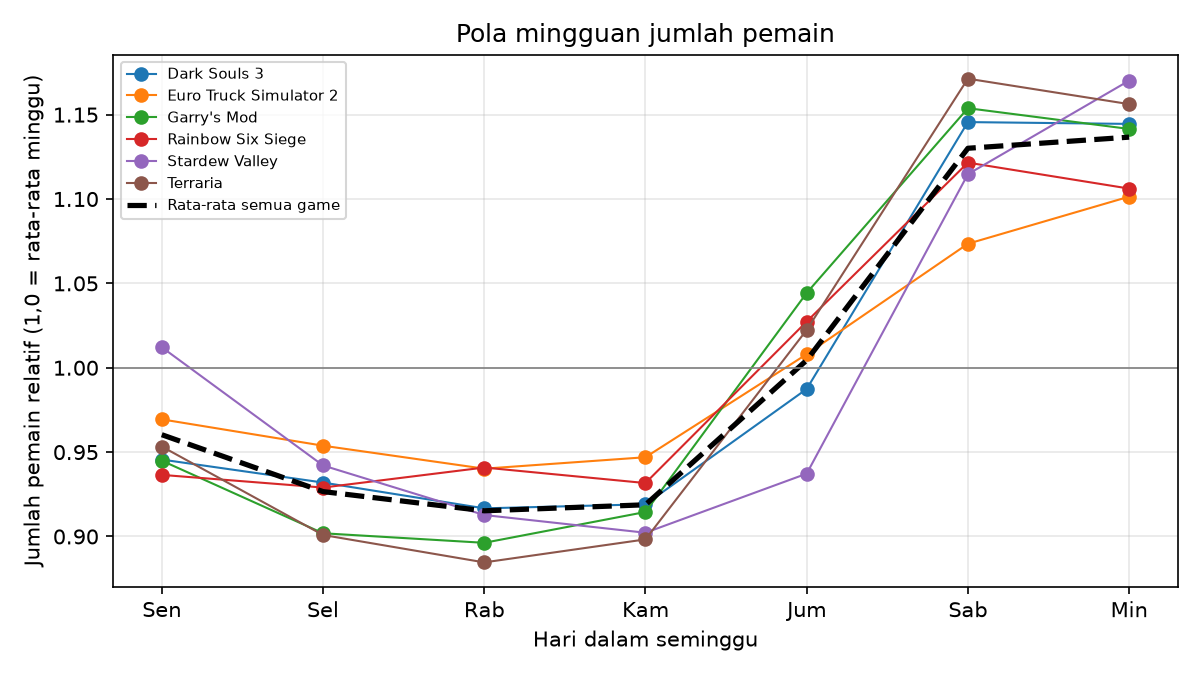
\includegraphics[width=0.92\columnwidth]{03_pola_mingguan.png}
\caption{Rata-rata jumlah pemain relatif per hari dalam seminggu. Nilai 1,0 berarti sama dengan rata-rata tujuh hari di sekitarnya.}
\label{fig:mingguan}
\end{figure}

Gambar~\ref{fig:mingguan} menunjukkan pola mingguan. Untuk menghilangkan pengaruh tren, jumlah pemain setiap hari dibagi dengan rata-rata tujuh hari di sekitarnya. Rata-rata keenam game mencapai 1,130 pada hari Sabtu dan 1,137 pada hari Minggu, sedangkan titik terendah ada pada hari Rabu (0,915). Pada setiap game, nilai Sabtu dan Minggu lebih tinggi daripada semua hari kerja.

\subsection{Hasil Encoding}

\begin{figure*}[t]
\centering
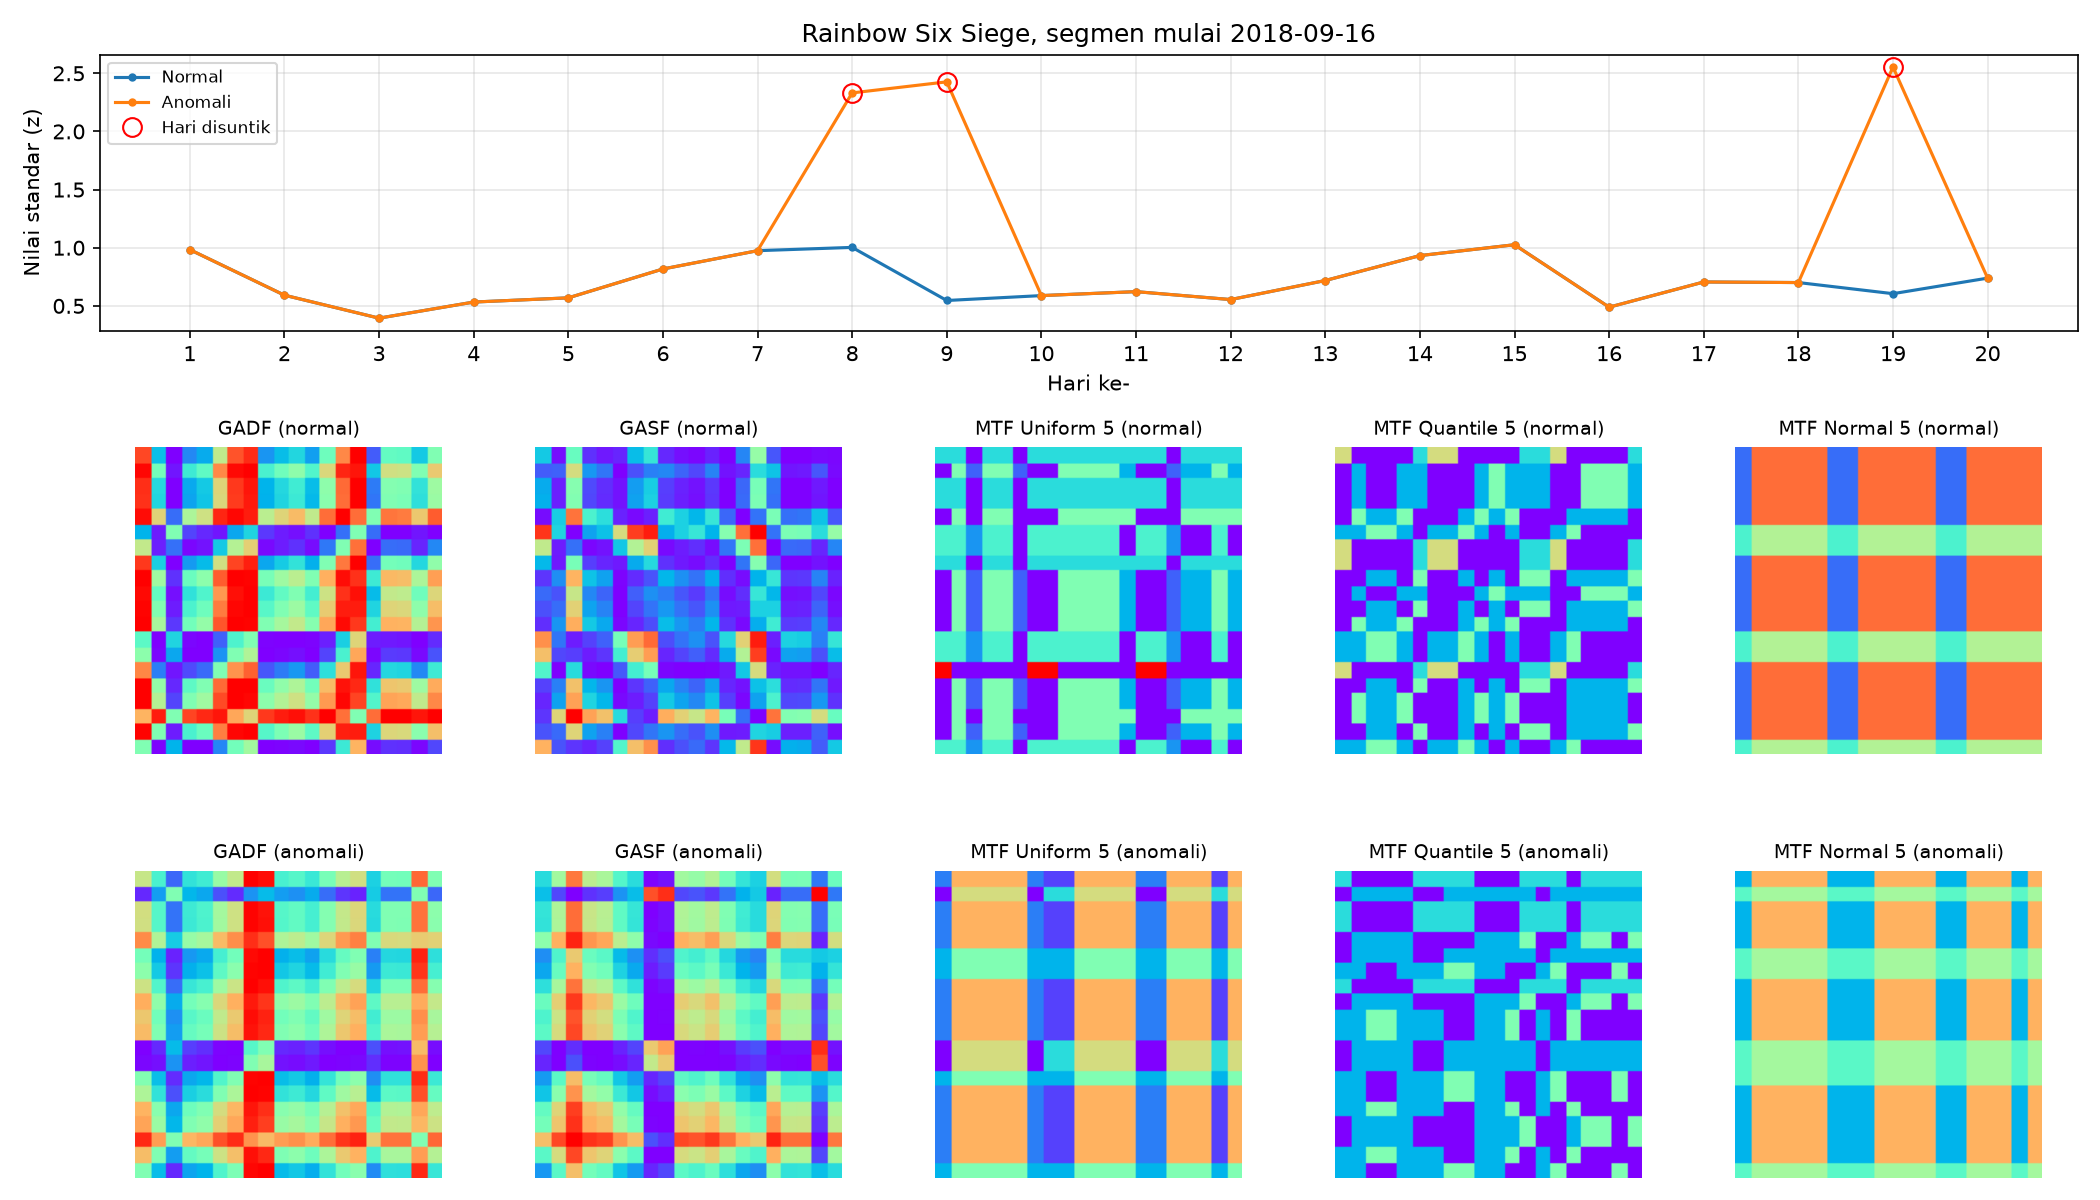
\includegraphics[width=0.66\textwidth]{05_pasangan_gambar_2.png}
\caption{Contoh segmen Rainbow Six Siege. Atas: deret waktu terstandar, dengan hari yang disuntik ditandai lingkaran merah. Tengah dan bawah: gambar dari segmen normal dan segmen anomali untuk lima encoding.}
\label{fig:pasangan}
\end{figure*}

Gambar~\ref{fig:pasangan} membandingkan gambar normal dan anomali untuk satu segmen. Pada GADF dan GASF, setiap hari yang disuntik menghasilkan garis tebal yang memotong gambar secara horizontal dan vertikal. Pada MTF Uniform, warna dominan gambar berubah. Sebaliknya, gambar MTF Quantile normal dan anomali terlihat mirip, karena pembagian bin pada strategi ini hanya bergantung pada urutan nilai dalam segmen, bukan pada besarnya.

\begin{table}[t]
\centering
\caption{Selisih statistik matriks antara data normal dan anomali}
\label{tab:delta}
\footnotesize
\begin{tabular}{lrrr}
\toprule
Encoding & \dmean & \dsd & \dcount \\
\midrule
GADF & 0,000 & 0,155 & 1,632 \\
GASF & 0,040 & 0,063 & 0,217 \\
MTF Uniform 2 & 0,165 & 0,036 & 0,015 \\
MTF Uniform 4 & 0,241 & 0,022 & 1,141 \\
MTF Uniform 5 & 0,268 & 0,033 & 1,149 \\
MTF Uniform 10 & 0,199 & 0,038 & 0,601 \\
MTF Quantile 2 & 0,000 & 0,061 & 0,124 \\
MTF Quantile 4 & 0,000 & 0,022 & 0,149 \\
MTF Quantile 5 & 0,000 & 0,014 & 0,211 \\
MTF Quantile 10 & 0,000 & 0,001 & 0,006 \\
MTF Normal 2 & 0,087 & 0,099 & 1,390 \\
MTF Normal 4 & 0,121 & 0,068 & 2,023 \\
MTF Normal 5 & 0,123 & 0,054 & 1,888 \\
MTF Normal 10 & 0,099 & 0,026 & 0,925 \\
\bottomrule
\end{tabular}
\end{table}

Tabel~\ref{tab:delta} merangkum selisih statistik matriks. Nilai \dmean{} GADF selalu nol karena matriks GADF antisimetris, dan \dmean{} MTF Quantile juga nol karena setiap bin selalu terisi sama banyak. Nilai \dcount{} pada GAF sangat kecil karena jumlah nilai unik pada matriks GADF dan GASF hampir selalu mendekati batas maksimumnya, baik untuk segmen normal maupun anomali (rata-rata 359,5 dan 361,1 untuk GADF, serta 208,3 dan 208,5 untuk GASF). Hal ini terjadi karena jumlah pemain harian hampir tidak pernah bernilai sama pada dua hari yang berbeda.

\begin{figure}[t]
\centering
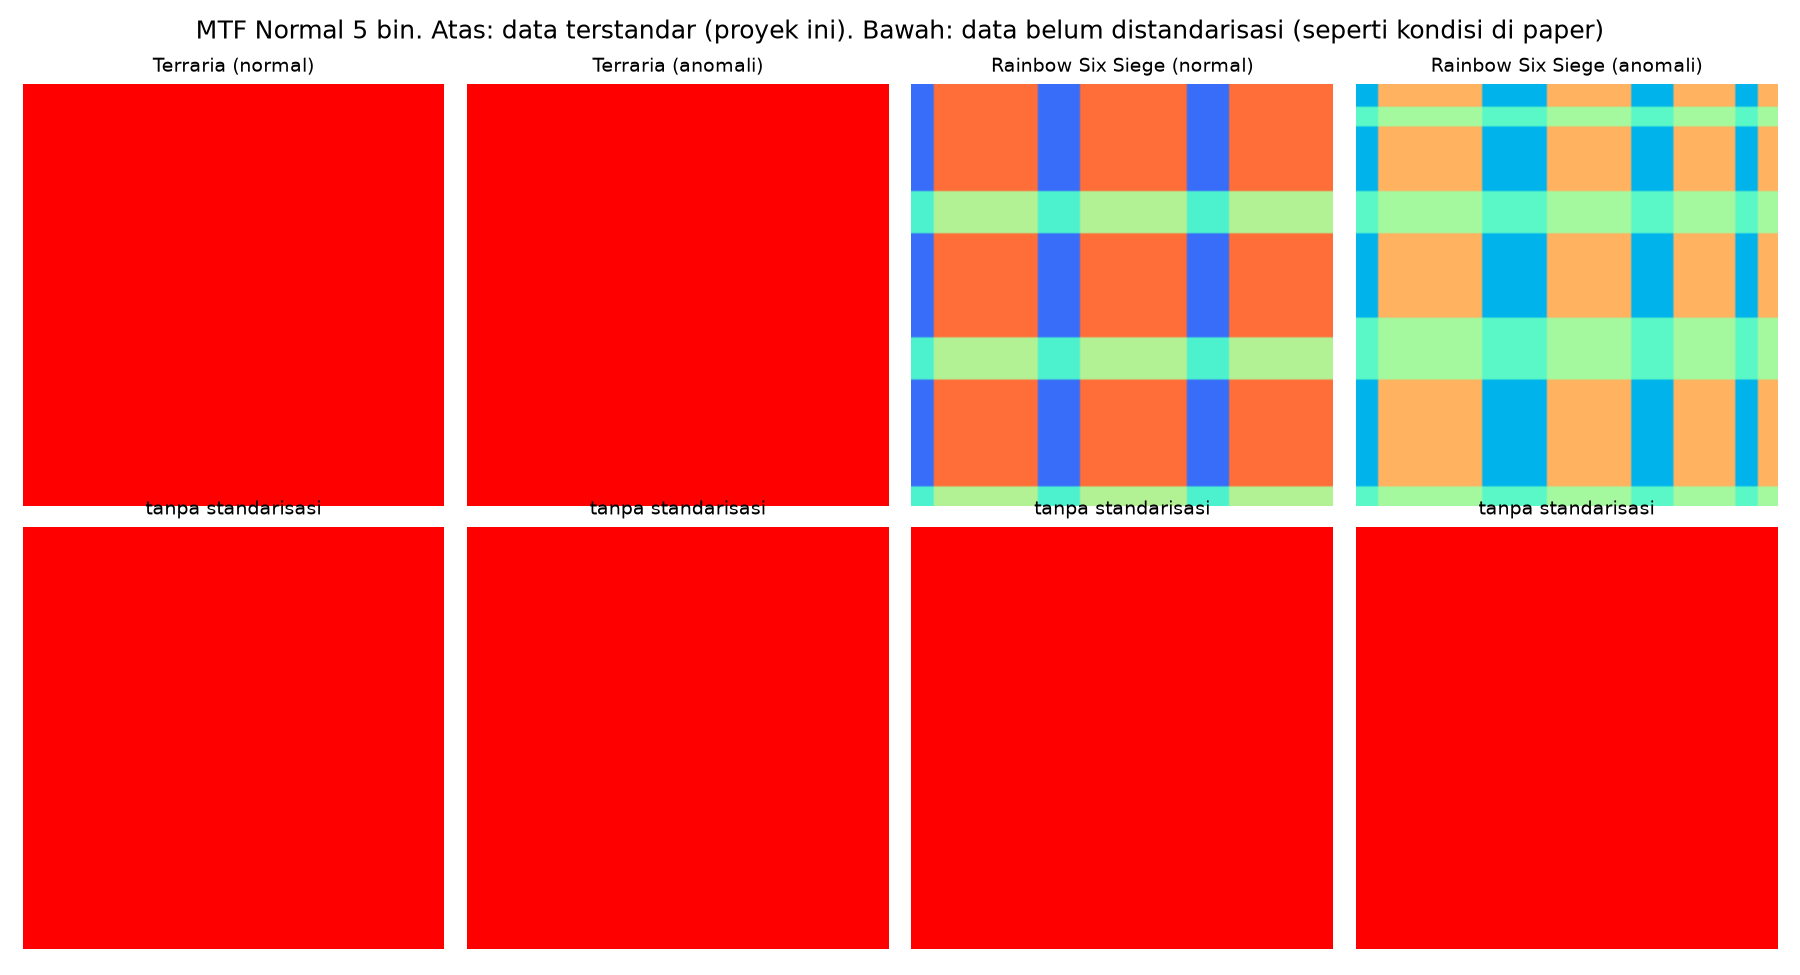
\includegraphics[width=0.9\columnwidth]{08_mtf_normal_standar_vs_mentah.png}
\caption{MTF Normal 5 bin. Atas: data terstandar seperti pada penelitian ini. Bawah: data yang belum distandarisasi, dengan seluruh gambar berwarna merah polos.}
\label{fig:mtfnormal}
\end{figure}

Hasil MTF Normal berbeda dari paper acuan, yang melaporkan bahwa seluruh gambar MTF Normal berwarna merah polos~\cite{rahadian2023}. Pada pustaka pyts, strategi normal memakai batas bin tetap dari distribusi normal baku tanpa menyesuaikan skala data. Jika semua nilai satu segmen jatuh ke bin yang sama, matriks hanya berisi angka 1 dan gambarnya menjadi merah polos. Karena data penelitian ini sudah distandarisasi, nilainya tersebar di sekitar nol sehingga melewati beberapa bin. Gambar~\ref{fig:mtfnormal} memperlihatkan perbedaan ini. Ketika MTF Normal diterapkan pada data yang hanya diubah ke $\log_{10}$ tanpa standarisasi, 100\% gambar menjadi seragam. Pada data terstandar, gambar seragam masih muncul, tetapi jauh lebih sering pada segmen normal daripada segmen anomali: 66,8\% berbanding 19,0\% untuk 2 bin, dan 8,5\% berbanding 2,5\% untuk 10 bin.

\begin{figure*}[t]
\centering
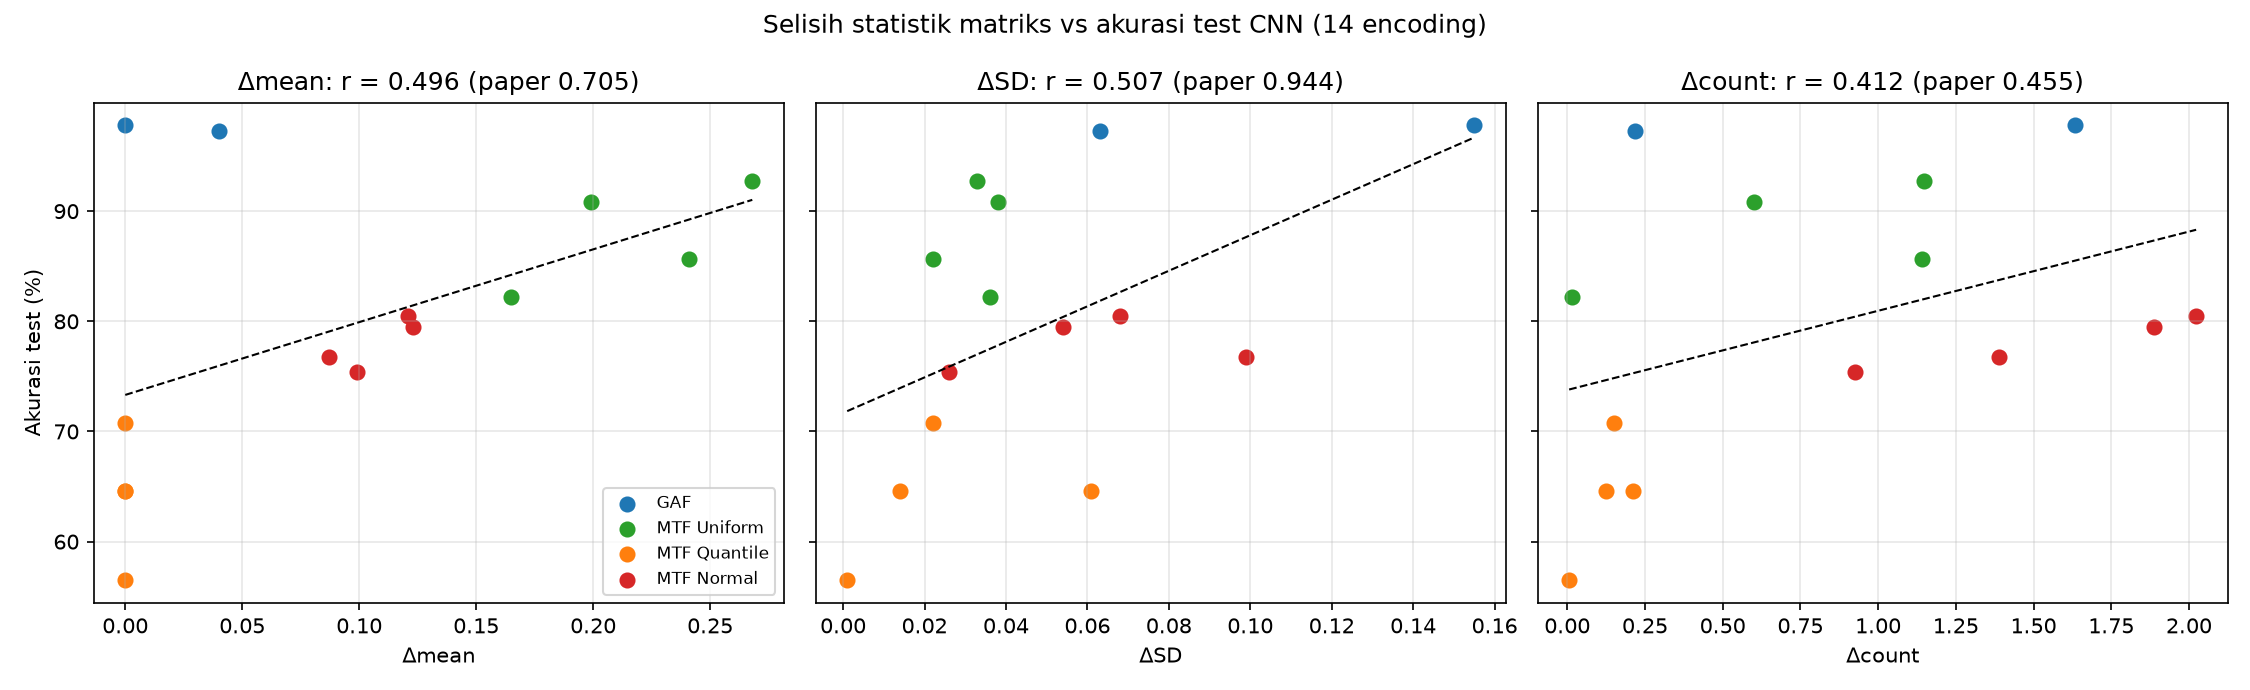
\includegraphics[width=0.82\textwidth]{12_korelasi_scatter.png}
\caption{Hubungan antara selisih statistik matriks dan akurasi test untuk 14 encoding. Garis putus-putus adalah garis regresi linear.}
\label{fig:scatter}
\end{figure*}

\subsection{Akurasi CNN}

\begin{table}[t]
\centering
\caption{Akurasi (\%) dan metrik data test untuk setiap encoding}
\label{tab:akurasi}
\footnotesize
\setlength{\tabcolsep}{3.5pt}
\begin{tabular}{lrrrrrr}
\toprule
Encoding & Train & Val & Test & Prec. & Recall & F1 \\
\midrule
GADF & 100,0 & 97,3 & 97,8 & 0,973 & 0,984 & 0,978 \\
GASF & 100,0 & 97,6 & 97,3 & 0,973 & 0,973 & 0,973 \\
MTF Uniform 2 & 97,1 & 84,2 & 82,2 & 0,829 & 0,811 & 0,820 \\
MTF Uniform 4 & 99,6 & 89,4 & 85,7 & 0,827 & 0,903 & 0,863 \\
MTF Uniform 5 & 99,9 & 92,1 & 92,7 & 0,939 & 0,914 & 0,926 \\
MTF Uniform 10 & 100,0 & 91,6 & 90,8 & 0,927 & 0,886 & 0,906 \\
MTF Quantile 2 & 80,1 & 67,9 & 64,6 & 0,665 & 0,589 & 0,625 \\
MTF Quantile 4 & 96,1 & 70,4 & 70,8 & 0,723 & 0,676 & 0,698 \\
MTF Quantile 5 & 97,3 & 70,4 & 64,6 & 0,650 & 0,632 & 0,641 \\
MTF Quantile 10 & 98,5 & 57,1 & 56,5 & 0,564 & 0,573 & 0,568 \\
MTF Normal 2 & 81,6 & 77,7 & 76,8 & 0,783 & 0,741 & 0,761 \\
MTF Normal 4 & 91,1 & 83,4 & 80,5 & 0,827 & 0,773 & 0,799 \\
MTF Normal 5 & 90,9 & 80,4 & 79,5 & 0,866 & 0,697 & 0,772 \\
MTF Normal 10 & 96,2 & 78,5 & 75,4 & 0,730 & 0,805 & 0,766 \\
\bottomrule
\end{tabular}
\end{table}

Tabel~\ref{tab:akurasi} menunjukkan bahwa GADF dan GASF memberikan akurasi test tertinggi, yaitu 97,8\% dan 97,3\%. Dari 370 gambar test, GADF hanya salah pada 8 gambar. Urutan berikutnya adalah MTF Uniform (82,2\% sampai 92,7\%), MTF Normal (75,4\% sampai 80,5\%), dan MTF Quantile (56,5\% sampai 70,8\%). Urutan keluarga encoding ini mirip dengan paper acuan, yang juga menempatkan GAF dan MTF Uniform di atas MTF Quantile~\cite{rahadian2023}, walaupun akurasi MTF Uniform pada data kami lebih rendah.

Selisih antara akurasi train dan test menunjukkan adanya overfitting pada sebagian besar encoding MTF. Contoh paling jelas adalah MTF Quantile 10 dengan akurasi train 98,5\% tetapi akurasi test hanya 56,5\%, serta MTF Normal 10 dengan 96,2\% berbanding 75,4\%. Pada GADF dan GASF selisihnya kecil (100\% berbanding 97,8\% dan 97,3\%). Karena pengaturan CNN sengaja disamakan dengan paper acuan, tidak ada regularisasi tambahan yang diberikan.

Akurasi MTF Normal berada di atas 50\%, berbeda dengan paper acuan. Analisis per gambar memperlihatkan bahwa sebagian akurasi ini berasal dari jalan pintas. Untuk 2 bin terdapat 149 gambar seragam pada data test, 120 di antaranya berasal dari segmen normal. CNN mengklasifikasikan gambar seragam dengan akurasi 80,5\%, yang sama dengan proporsi segmen normal di antara gambar seragam tersebut. Artinya, CNN menebak ``normal'' untuk setiap gambar merah polos. Pola yang sama terlihat untuk 4, 5, dan 10 bin. Pada gambar yang tidak seragam, akurasinya 74,2\% sampai 79,4\%.

Dari sisi waktu, training memerlukan rata-rata 41,2 detik per encoding, sedangkan pembuatan matriks dan gambar untuk 2.458 segmen kurang dari 0,25 detik. Seperti pada paper acuan~\cite{rahadian2023}, training CNN adalah bagian yang paling memakan waktu.

\begin{figure*}[t]
\centering
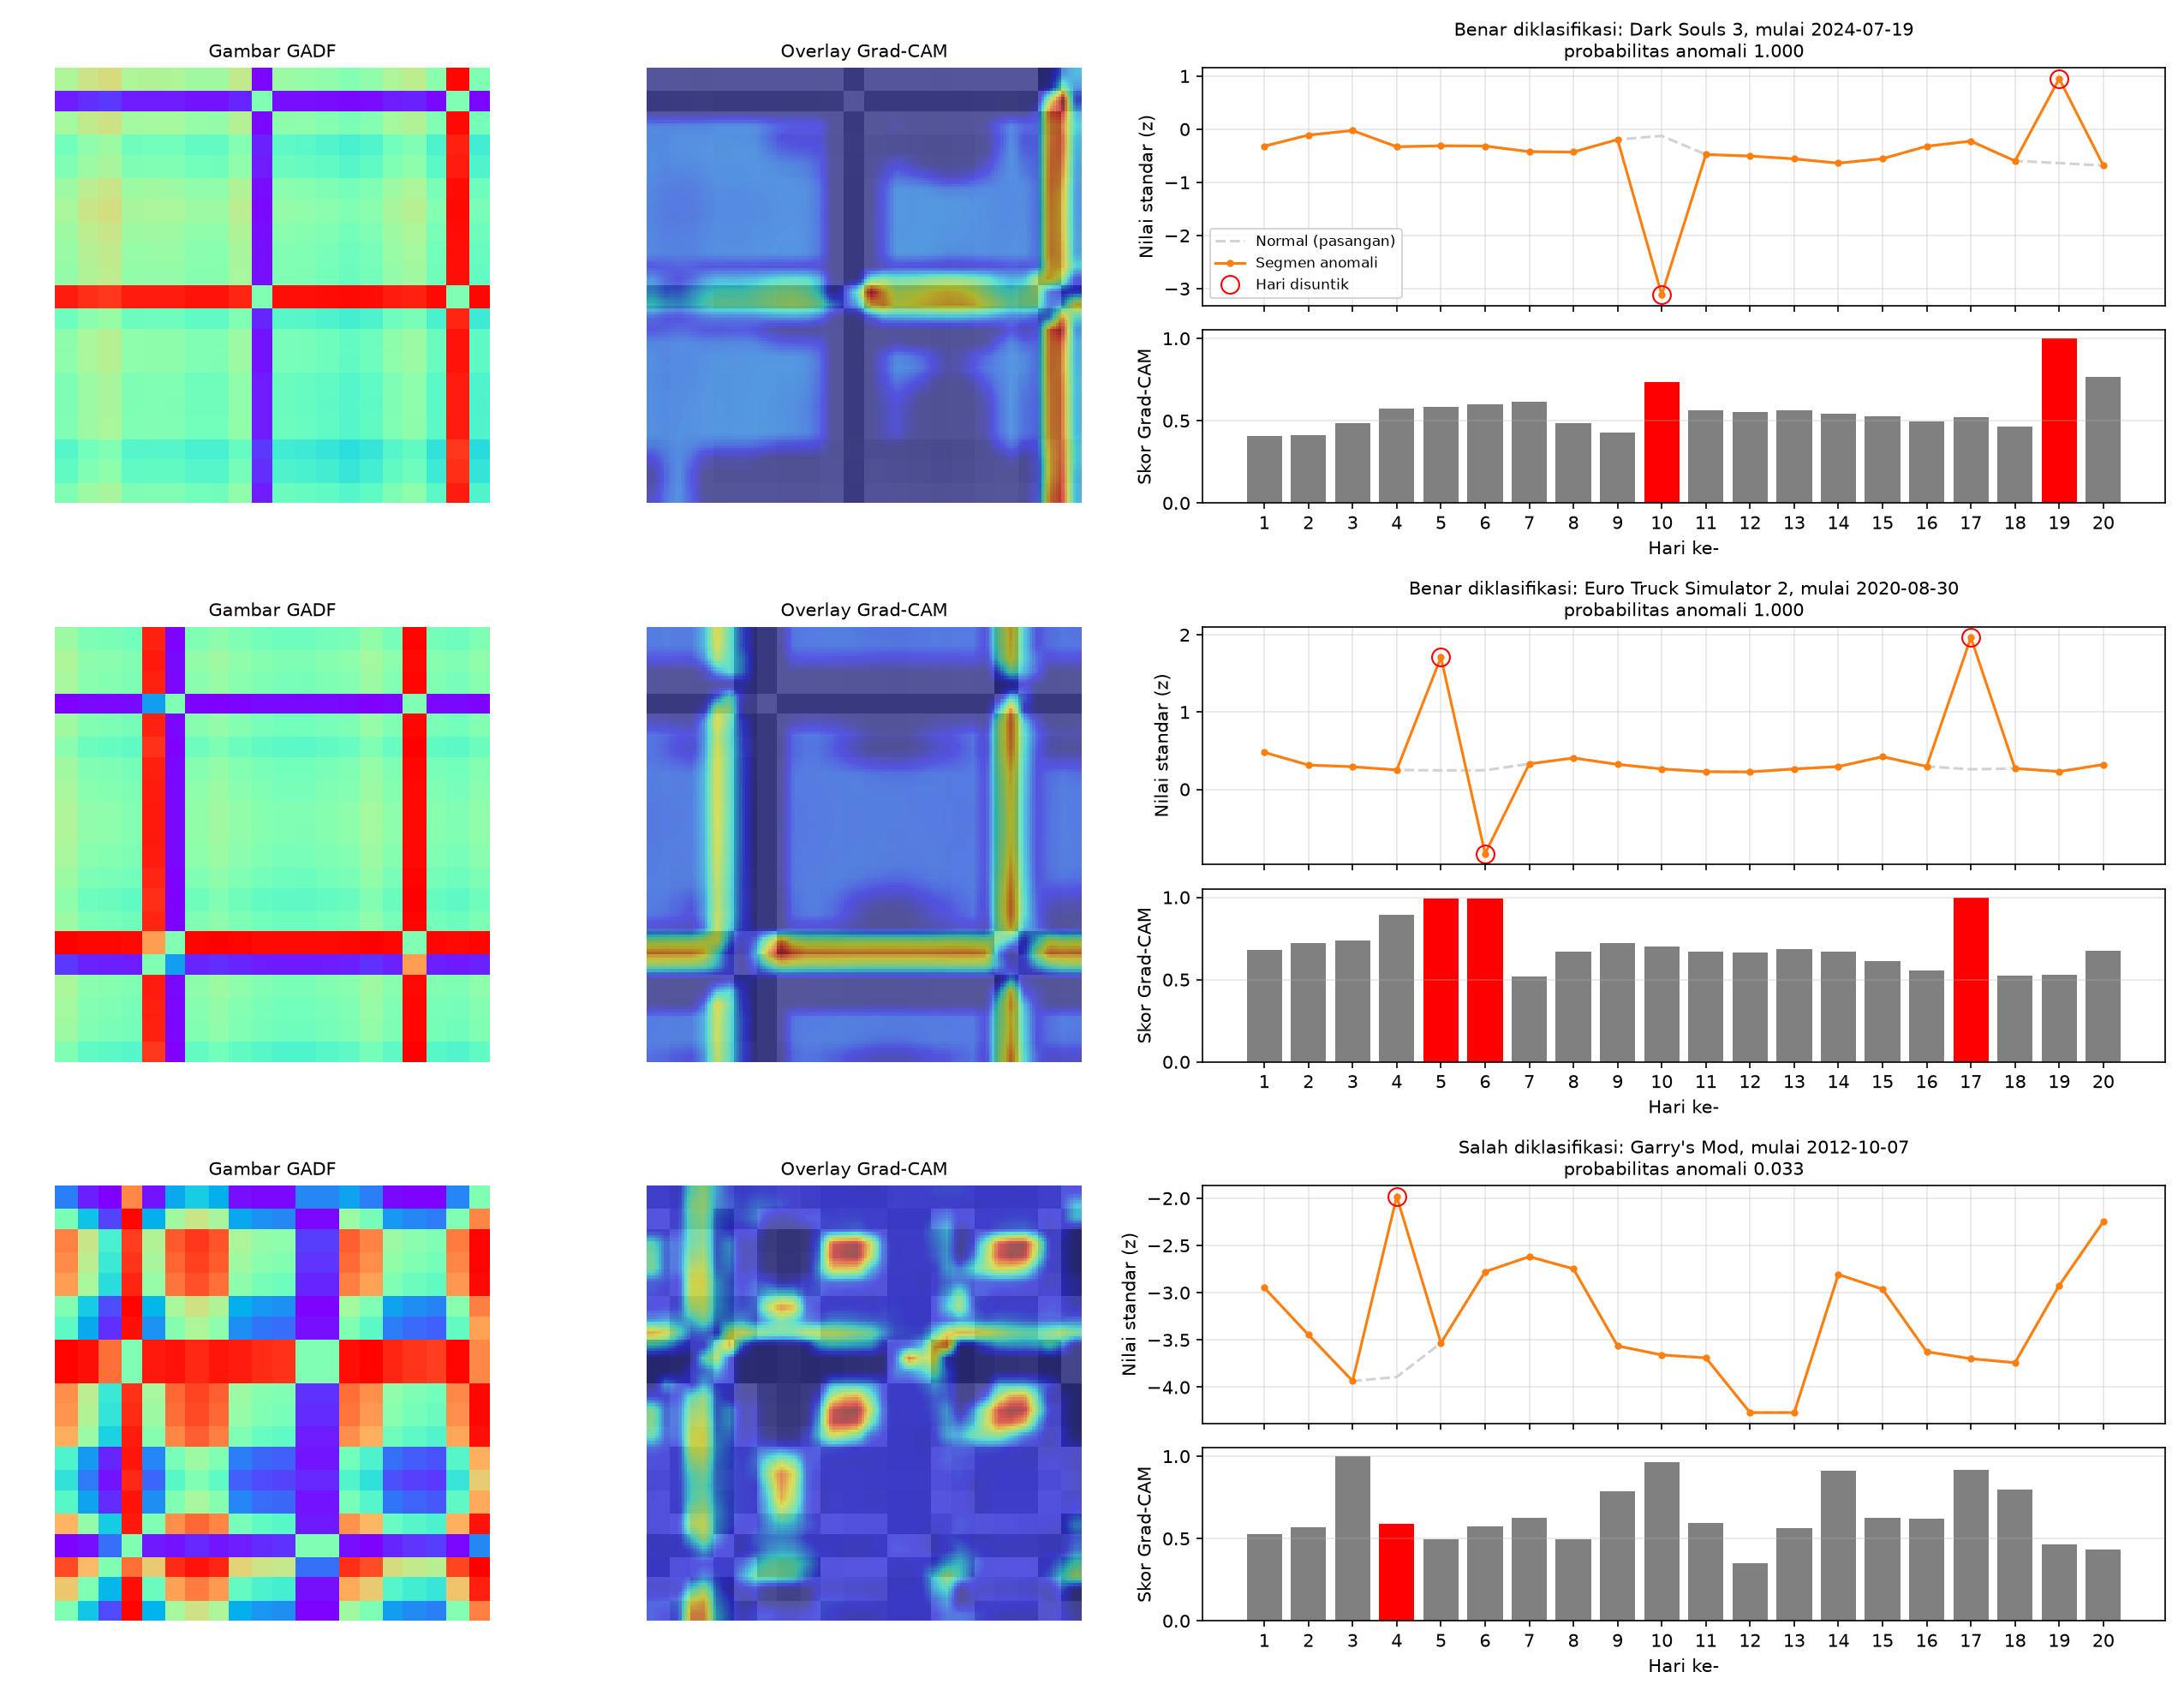
\includegraphics[width=0.6\textwidth]{13_gradcam_contoh.png}
\caption{Grad-CAM pada model GADF untuk tiga segmen anomali dari data test. Kolom kiri ke kanan: gambar GADF, overlay Grad-CAM, deret waktu (lingkaran merah menandai hari yang disuntik), dan skor Grad-CAM per hari (batang merah adalah hari yang disuntik).}
\label{fig:gradcam}
\end{figure*}

\subsection{Korelasi Pearson}

\begin{table}[t]
\centering
\caption{Korelasi Pearson antara selisih statistik dan akurasi test}
\label{tab:korelasi}
\begin{tabular}{lrr}
\toprule
Fitur & $r$ penelitian ini & $r$ paper acuan~\cite{rahadian2023} \\
\midrule
\dmean & 0,496 & 0,705 \\
\dsd & 0,507 & 0,944 \\
\dcount & 0,412 & 0,455 \\
\bottomrule
\end{tabular}
\end{table}

Tabel~\ref{tab:korelasi} dan Gambar~\ref{fig:scatter} membandingkan korelasi pada data ini dengan paper acuan. Urutan nilainya sama, yaitu \dsd{} tertinggi diikuti \dmean{} dan \dcount, tetapi kekuatannya berbeda. Nilai \dsd{} (0,507) dan \dmean{} (0,496) hampir sama, dan dengan hanya 14 titik selisih sekecil itu tidak dapat dianggap bermakna. Korelasi \dsd{} juga jauh lebih lemah daripada 0,944 pada paper acuan.

Ada beberapa kemungkinan penyebab perbedaan ini. Pertama, MTF Uniform mencapai akurasi 82,2\% sampai 92,7\% walaupun nilai \dsd-nya hanya 0,022 sampai 0,038. Kekuatan MTF Uniform pada data ini tampaknya berasal dari \dmean{} yang besar, sehingga titik-titiknya berada jauh di atas garis regresi \dsd. Kedua, pada paper acuan keempat varian MTF Normal memiliki semua selisih bernilai nol dengan akurasi 50\%~\cite{rahadian2023}. Kelompok titik ini kemungkinan ikut memperkuat korelasi. Pada data kami MTF Normal tidak berada di titik tersebut, sehingga pola yang rapi itu tidak muncul. Ketiga, \dmean{} bernilai nol untuk encoding terbaik (GADF) maupun terburuk (MTF Quantile), sehingga \dmean{} tidak dapat membedakan keduanya. Keempat, \dcount{} pada GAF hampir konstan seperti dijelaskan sebelumnya. Hanya \dcount{} yang korelasinya mendekati paper acuan (0,412 berbanding 0,455).

\subsection{Grad-CAM}

Grad-CAM diterapkan pada model GADF karena akurasi test-nya tertinggi. Dari 185 segmen anomali pada data test, model ini mengklasifikasikan 182 segmen dengan benar. Gambar~\ref{fig:gradcam} menampilkan dua contoh yang benar dan satu contoh yang salah, dipilih secara acak dengan seed tetap. Pada contoh ETS2 (segmen mulai 30 Agustus 2020), tiga hari dengan skor Grad-CAM tertinggi adalah hari ke-5, 6, dan 17, sama persis dengan tiga hari yang disuntik. Pada contoh Dark Souls 3 (mulai 19 Juli 2024), hari yang disuntik adalah hari ke-10 dan 19, sedangkan dua skor tertinggi jatuh pada hari ke-19 dan 20. Hari ke-20 kemungkinan ikut terang karena bertetangga dengan hari ke-19 dan peta Grad-CAM memiliki resolusi yang lebih rendah daripada gambar. Pada kedua contoh ini, area yang disorot adalah garis silang pada gambar GADF yang bersesuaian dengan hari anomali.

Contoh yang salah berasal dari Garry's Mod (mulai 7 Oktober 2012). Hari yang disuntik hanya hari ke-4, dan model memberikan probabilitas anomali 0,033. Peta Grad-CAM-nya tersebar ke banyak area dan skor tertinggi jatuh pada hari ke-3. Deret waktu segmen ini sudah naik turun cukup besar secara alami, sehingga satu hari lonjakan buatan tidak terlihat menonjol.

\section{Insight}

Bagian ini merangkum pelajaran yang dapat diambil dari hasil di atas.

\textbf{Akhir pekan adalah ritme dasar jumlah pemain.} Pola Sabtu dan Minggu yang lebih ramai muncul di keenam game, padahal genre dan usia game-nya sangat berbeda. Artinya, pola ini lebih ditentukan oleh waktu luang pemain daripada oleh jenis game. Bagi deteksi anomali, hal ini berarti segmen normal pun tidak datar, karena satu segmen 20 hari selalu memuat hampir tiga siklus mingguan. Sebuah metode harus mampu membedakan naik turun mingguan yang wajar dari perubahan yang benar-benar tidak biasa.

\textbf{GAF unggul karena satu hari anomali menjadi pola yang mudah dilihat.} Pada GAF, satu hari yang berubah memengaruhi seluruh baris dan kolom hari tersebut, sehingga anomali yang hanya terjadi satu hari berubah menjadi garis silang yang membentang di seluruh gambar. Pola seperti ini mudah dikenali oleh CNN. Grad-CAM memperlihatkan bahwa pada contoh yang benar CNN memang memperhatikan garis tersebut, dan karena posisi garis bersesuaian dengan nomor hari, keputusan CNN dapat dipetakan kembali ke tanggal pada data aslinya.

\textbf{Encoding perlu menjaga informasi yang membedakan anomali.} Anomali pada penelitian ini adalah perubahan besar dalam jumlah pemain. MTF Quantile hanya melihat urutan nilai, sehingga lonjakan dua kali lipat dan lima kali lipat dapat menghasilkan gambar yang sama. Encoding yang mempertahankan besarnya nilai, seperti GAF dan MTF Uniform, lebih cocok untuk jenis anomali ini.

\textbf{Akurasi yang tinggi belum tentu berarti CNN memahami pola.} Standarisasi data membuat MTF Normal tidak lagi menghasilkan gambar merah polos untuk semua segmen, sehingga hasilnya berbeda dari paper acuan karena perbedaan pra-pemrosesan data. Namun, sebagian akurasinya berasal dari jalan pintas: CNN menebak ``normal'' untuk setiap gambar polos. Hal ini menunjukkan pentingnya memeriksa isi gambar dan cara model mengambil keputusan, bukan hanya melihat angka akurasi.

\textbf{Pemilihan encoding lewat statistik matriks perlu disesuaikan dengan karakter data.} Pada data tegangan di paper acuan, \dsd{} sangat kuat menunjukkan encoding yang baik~\cite{rahadian2023}. Pada data jumlah pemain, hubungannya jauh lebih lemah. Data kami memiliki nilai harian yang hampir tidak pernah berulang dan anomali yang dapat naik maupun turun, sehingga statistik matriks berperilaku berbeda. Statistik matriks tetap berguna sebagai penyaring awal, misalnya untuk menyingkirkan encoding yang semua selisihnya kecil, tetapi pada data seperti ini hasilnya sebaiknya tetap dipastikan dengan percobaan CNN.

\textbf{Data nyata sudah mengandung lonjakan yang mirip anomali.} Sekitar sepersepuluh segmen normal, dan seperlima segmen Terraria, sudah memuat lonjakan alami. Anomali buatan yang besarnya mirip dengan variasi alami sulit dikenali, seperti pada contoh Garry's Mod yang salah diklasifikasi. Dengan kata lain, apa yang disebut ``normal'' pada data jumlah pemain tidak selalu tenang, dan label anomali buatan tidak dapat menangkap semua kejadian yang sebenarnya tidak biasa.

\section{Kesimpulan}

Penerapan metode Rahadian dkk.~\cite{rahadian2023} pada data jumlah pemain harian enam game Steam menunjukkan bahwa GADF dan GASF adalah encoding terbaik (97,8\% dan 97,3\%), dan Grad-CAM memperlihatkan bahwa CNN memperhatikan hari anomali pada gambar GADF. Urutan korelasi statistik matriks sama dengan paper acuan, tetapi korelasi \dsd{} jauh lebih lemah (0,507 berbanding 0,944), sehingga pada data ini pemilihan encoding hanya dari statistik matriks kurang dapat diandalkan. Dari sisi data, jumlah pemain pada akhir pekan konsisten lebih tinggi di semua game.

Penelitian ini memiliki beberapa keterbatasan. Anomali yang dipakai adalah anomali buatan, sehingga belum tentu mewakili kejadian nyata seperti pembaruan besar atau gangguan server. Sebagian besar encoding MTF mengalami overfitting karena pengaturan CNN sengaja disamakan dengan paper acuan tanpa regularisasi. Setiap encoding hanya dilatih satu kali, dan data test hanya berisi 370 gambar, sehingga selisih akurasi beberapa poin antar encoding sebaiknya tidak ditafsirkan berlebihan. Penelitian berikutnya dapat mengulang training dengan beberapa seed, menambahkan regularisasi, dan menguji metode ini pada anomali nyata yang diberi label secara manual.


\bibliographystyle{IEEEtran}
\bibliography{refs}

\end{document}
